% !TEX root = main.tex

\section{Exercise 4}
\subsection{Continuous time state space model}
We introduce two new states (elevation $e$ and its rate $\dot{e}$) in order to be able to control them. The continuous time system can now be written as $\mathbf{\dot{x}} = \mathbf{A}_c\mathbf{x}+ \mathbf{B}_c \mathbf{u}$, with
\begin{subequations}
    \begin{align}
        \mathbf{x} &= \begin{bmatrix}
            \lambda\\
            r\\
            p\\
            \dot{p}\\
            e\\
            \dot{e}\\
        \end{bmatrix}\\
        \mathbf{u} &= \begin{bmatrix}
            p_c\\
            e_c\\
        \end{bmatrix}\\
    \mathbf{A_c} &= \begin{bmatrix}
        0 & 1 & 0          & 0          & 0          & 0         \\
        0 & 0 & -K_2       & 0          & 0          & 0         \\
        0 & 0 & 0          & 1          & 0          & 0         \\
        0 & 0 & -K_1K_{pp} & -K_1K_{pd} & 0          & 0         \\
        0 & 0 & 0          & 0          & 0          & 1         \\
        0 & 0 & 0          & 0          & -K_3K_{ep} & -K_3K_{ed}
    \end{bmatrix}\\
    \mathbf{B_c} &= \begin{bmatrix}
        0         & 0        \\
        0         & 0        \\
        0         & 0        \\
        K_1K_{pp} & 0        \\
        0         & 0        \\
        0         & K_3K_{ep}
    \end{bmatrix}
    \end{align}
\end{subequations}
\subsection{Discrete time state space model}
The system was discretized using the forward Euler method. Using \cref{eq:eulerfwd}, we get the model $\mathbf{x_{k+1}} = \mathbf{A}_d\mathbf{x_k}+\mathbf{B}_d \mathbf{u_k}$, where
\begin{subequations}
    \begin{align}
    \mathbf{A_d} &= \begin{bmatrix}
        1 & h & 0           & 0            & 0           & 0         \\
        0 & 1 & -hK_2       & 0            & 0           & 0         \\
        0 & 0 & 1           & h            & 0           & 0         \\
        0 & 0 & -hK_1K_{pp} & 1-hK_1K_{pd} & 0           & 0         \\
        0 & 0 & 0           & 0            & 1           & h         \\
        0 & 0 & 0           & 0            & -hK_3K_{ep} & 1-hK_3K_{ed}
    \end{bmatrix}\\
    \mathbf{B_d} &= \begin{bmatrix}
        0          & 0        \\
        0          & 0        \\
        0          & 0        \\
        hK_1K_{pp} & 0        \\
        0          & 0        \\
        0          & hK_3K_{ep}
    \end{bmatrix}
    \end{align}
\end{subequations}

\subsection{Objective function and inequality constraints on elevation}
In this exercise, we minimized the cost function
\begin{equation}
        \phi =\sum (\lambda_i - \lambda_f)^2 + r_{p}p_{ci}^2 + r_{e}e_{ci}^2
\end{equation}
which can be written as
\begin{subequations}
    \begin{align}
        \phi &= \sum(x^{T}\mathbf{Q}x+u^{T}\mathbf{R}u) \\
        \mathbf{Q} &= \begin{bmatrix}
        1 & 0 & 0 & 0 & 0 & 0         \\
        0 & 0 & 0 & 0 & 0 & 0         \\
        0 & 0 & 0 & 0 & 0 & 0         \\
        0 & 0 & 0 & 0 & 0 & 0         \\
        0 & 0 & 0 & 0 & 0 & 0         \\
        0 & 0 & 0 & 0 & 0 & 0
        \end{bmatrix}\\
        \mathbf{R} &= \begin{bmatrix}
            q_1        & 0        \\
            0          & q_2
        \end{bmatrix}
    \end{align}
\end{subequations}
Having the cost function on this form makes it very easy to change or add weighting for different states and inputs.

We restricted the helicopter to obey the non-linear inequality constraint
\begin{equation}
e_k \geq \alpha e^{-\beta(\lambda_k-\lambda_t)^{2}}
\end{equation}
every timestep $k$ until the time horizon.
Since this constraint is non-linear, a non-linear solver was needed. The matlab function \texttt{fmincon} was used to compute the optimal trajectory through the state space.

%\todo[inline]{MAYBE ADD EXPLAIN FMINCON SOLUTION METHOD?}

%\todo[inline]{ADD PLOTS OF THE OPTIMAL PATH!! Done}
\begin{figure}
    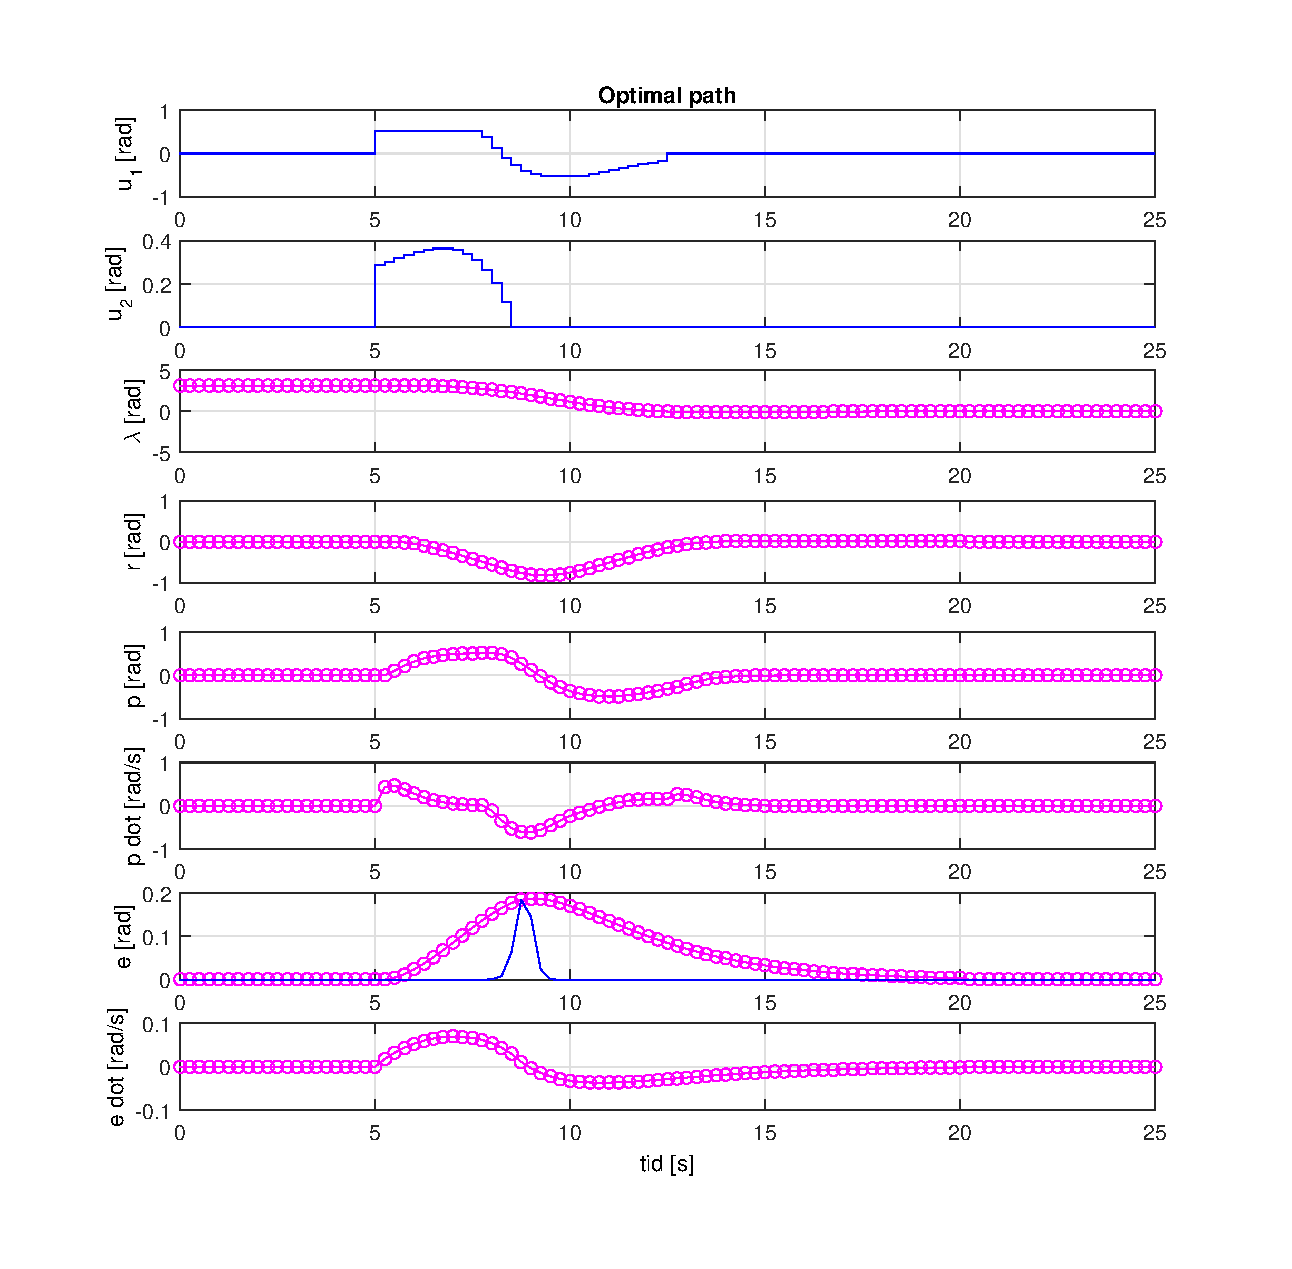
\includegraphics[width=\textwidth]{p4_trajectory.eps}
    \caption{Optimal trajectory in exercise 4. Evaluated constraint can be seen in blue in the elevation graph.}
    \label{fig:p4o}
\end{figure}

\begin{figure}
    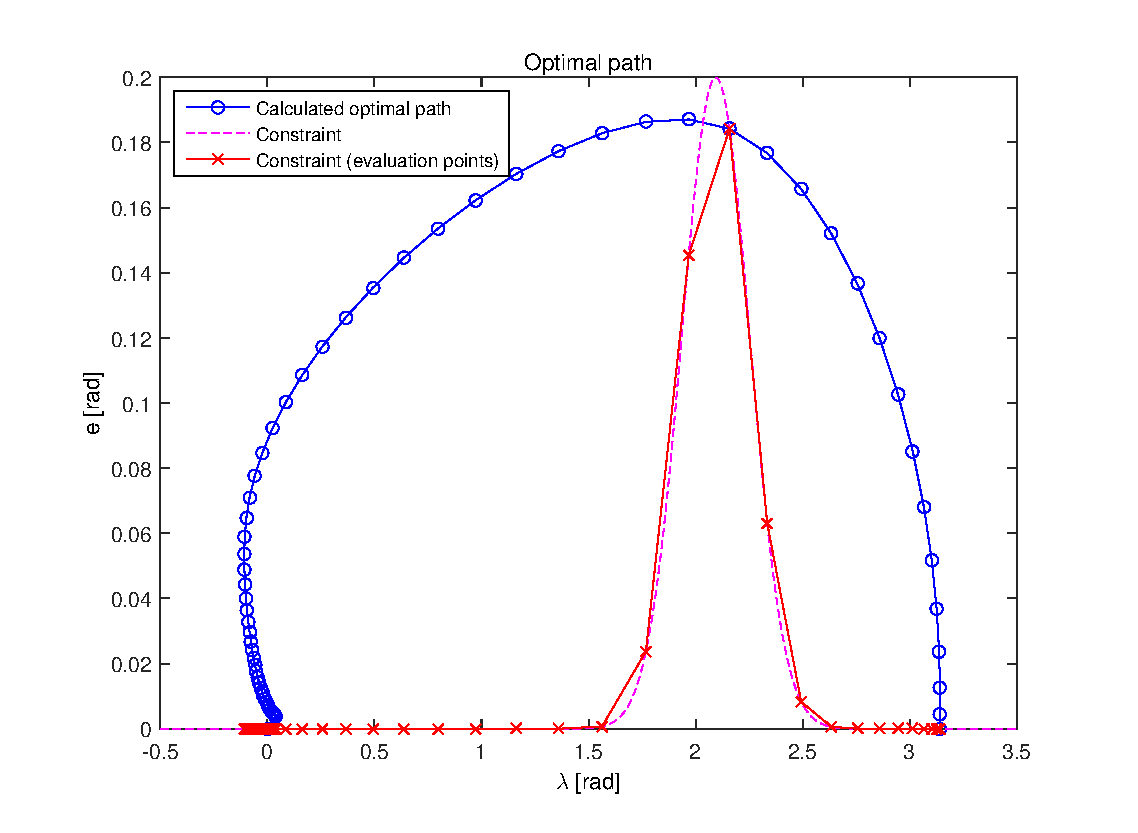
\includegraphics[width=\textwidth]{p4_2d_path.eps}
    \caption{Optimal trajectory in exercise 4. Evaluated constraint can be seen in blue in the elevation graph.}
    \label{fig:p4o2}
\end{figure}


%\todo[inline]{DISCUSS RESULTS!! Done here:}
The calculated optimal trajectory, shown in \cref{fig:p4o}, looks much like the one from \cref{subsec:p2o}. The elevation trajectory is also calculated, and appears to adhere to our constraint. Upon closer inspection, however, it is revealed that the trajectory passes through the constraint. This is because the discretization is too coarse to catch the ``collision'' (see \cref{fig:p4o2}).

\subsection{Experimental results}
The optimal trajectory was fed into the helicopter, both with and without feedback

%\todo[inline]{ADD PLOTS OF THE EXPERIMENT PATH!! WITH AND WITHOUT FEEDBACK}
\begin{figure}
    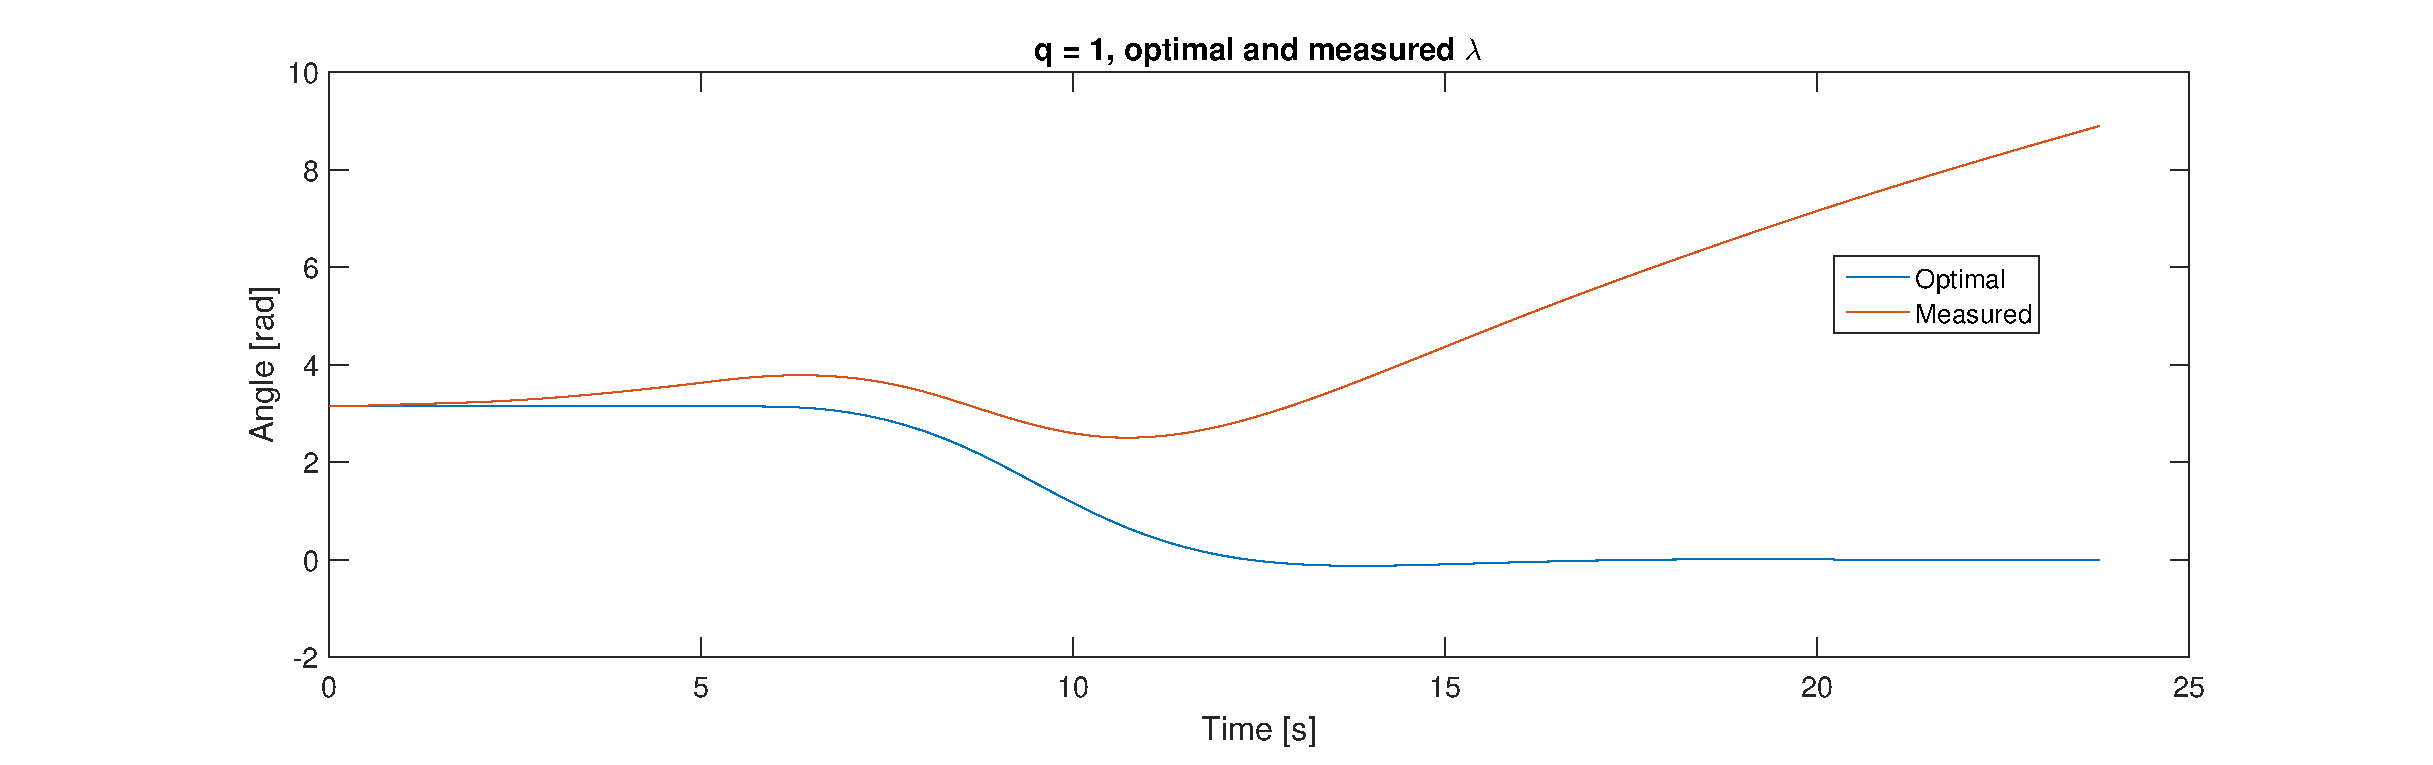
\includegraphics[width=\textwidth]{optimal_and_measured_lambda.eps}
    \caption{Optimal and measured travel and elevation over time.}
    \label{fig:p4d}
\end{figure}

\begin{figure}
    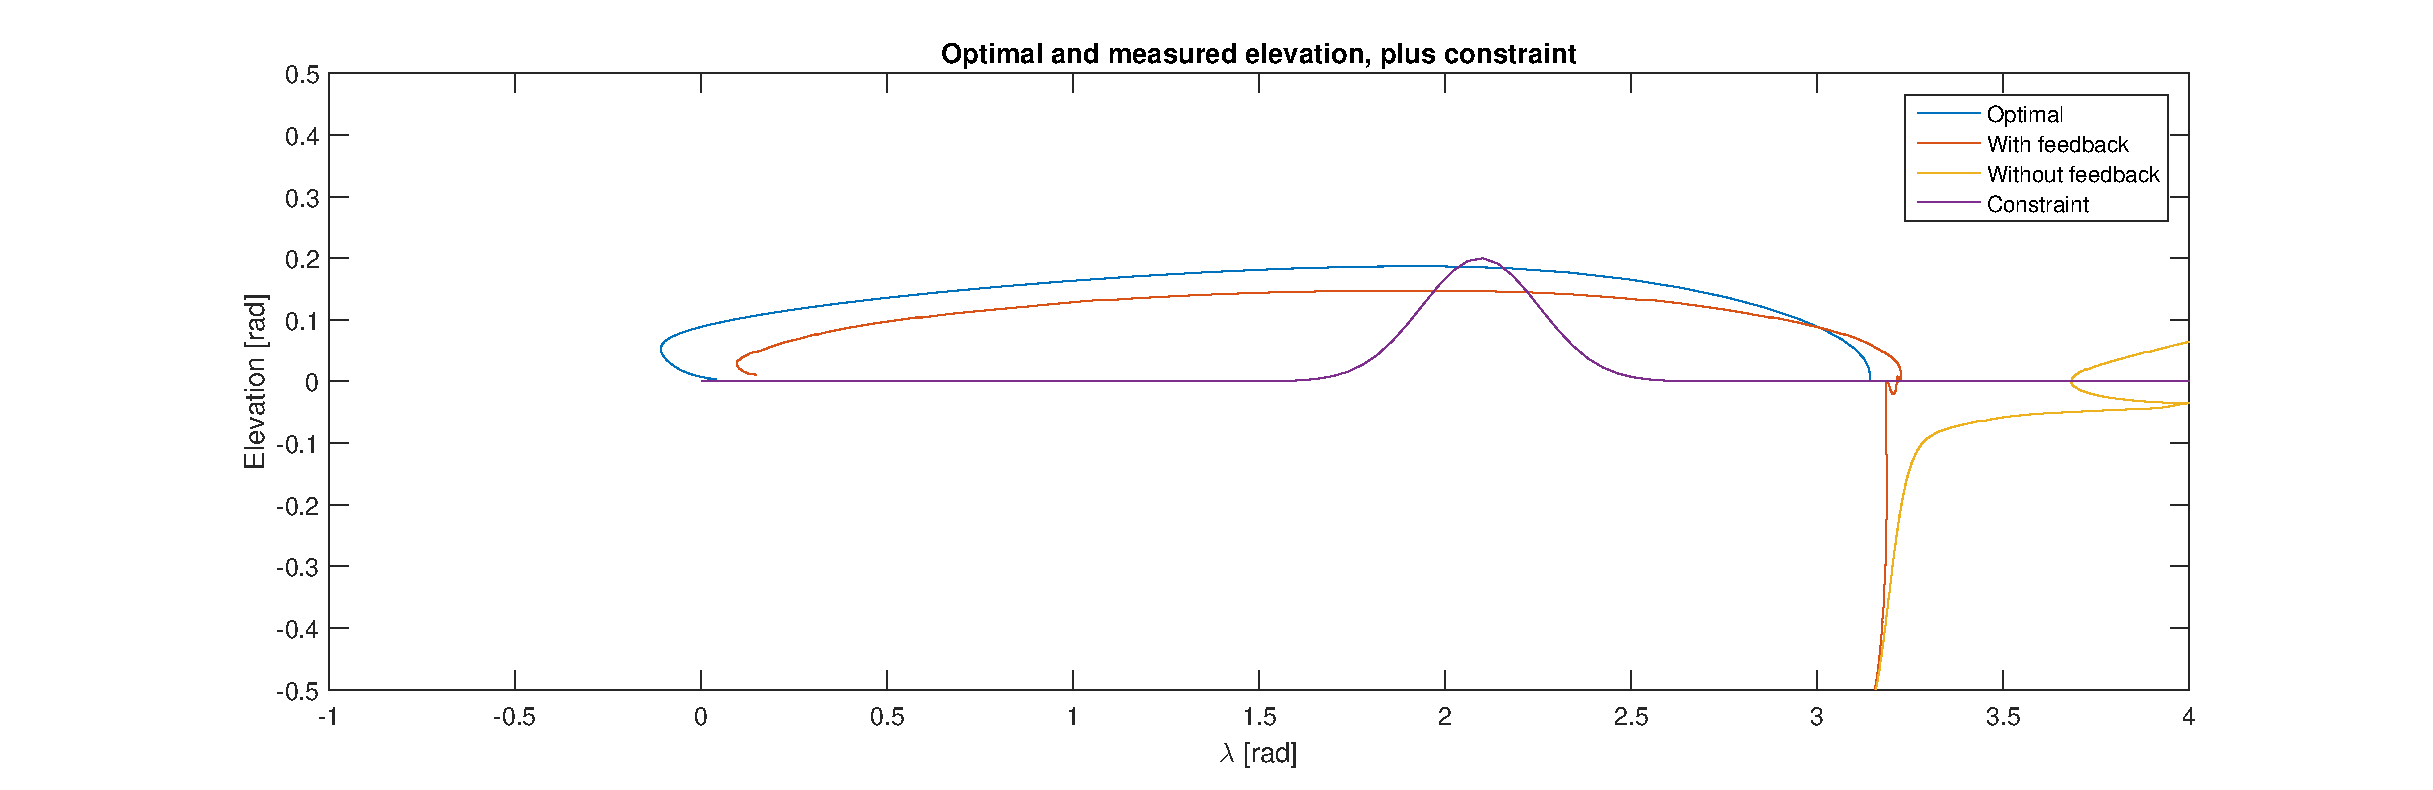
\includegraphics[width=\textwidth]{elevation_vs_lambda.eps}
    \caption{Optimal and measured travel against elevation with continuous constraint.}
    \label{fig:p4d2}
\end{figure}
%\todo[inline]{DISCUSS RESULTS!! Done here:}
The open-loop results, shown in \cref{fig:p4d} and \cref{fig:p4d2}, look much like the ones from \cref{subsec:p2d}, and measured $\lambda$ drifting off because of the lack of feedback. Measured $e$ was closer to following the path, because that state has its own controller with feedback anyway.

The closed loop results, however, go to the target position. While developing a relatively small constant error, the system reaches the target. It fails to stay entirely above the constraint. This is partially because the calculated optimal path travels through it, but also because the controller is not fast and accurate enough at that scale, and because the model is inaccurate. If the constraint represented an obstacle or hazard, it would have to be avoided by adding a bigger ``buffer zone''. Alternatively, an MPC controller could be used, allowing new paths avoiding the constraint to be calculated online.

\subsection{Decoupled states}
%\todo[inline]{ADD INFO ABOUT DECOUPLED STATES!! Done here:}
In the model used in this exercise, the elevation and pitch/travel systems are completely decoupled. This is obviously not true, as tilting the helicopter makes it harder to fly upwards, resulting in an inaccurate model. The model could include crossing terms accounting for this coupling, but that would make the objective function non-linear, making the problem a lot harder, computationally.